\section{The jj-coupling scheme}

\begin{frame}{The jj-coupling scheme}
\uncover<1->{
    \begin{block}{Hamiltonian}
        $H_{\mathrm{s-o}}\gg H_{\mathrm{re}}$:
        \begin{equation*}
            \begin{aligned}
                H&=H_{\mathrm{CF}}+H_{\mathrm{s-o}}\\
                &=\sum_{i=1}^N\left\{-\frac{\hbar^2}{2m}\nabla_i^2+V_{\mathrm{CF}}\left(r_i\right)\right\}+\sum_{i=1}^N \xi_i(r_i)\boldsymbol{l}_1\cdot\boldsymbol{s}_i\\
                &=\sum_{i=1}^N\left\{-\frac{\hbar^2}{2m}\nabla_i^2+V_{\mathrm{CF}}\left(r_i\right)+ \xi_i(r_i)\boldsymbol{l}_1\cdot\boldsymbol{s}_i\right\}.
            \end{aligned}
        \end{equation*}
        \uncover<2->{
        Approximate to an independent particle system.}
    \end{block}}
\uncover<3->{
    Use a complete set of quantum numbers for each electron to characterize quantum states: eigenstates of $H_{\mathrm{s-o}}$: $\prod\limits_i^N\ket{n_i l_i j_i (m_j)_i}$.
    }
\end{frame}

\begin{frame}{The jj-coupling scheme}
\uncover<1->{
    Energy:
    \begin{equation*}
        \begin{aligned}
            E_{\mathrm{s-o}}&=\sum_{i}^{N} \expval{H_{\mathrm{s-o}}}{n_i l_i j_i (m_j)_i}\\
            &=\frac{1}{2}\sum_{i}^{N} \xi_{in_il_i}(r_i)[j_i(j_i+1)-l_i(l_i+1)-\frac{3}{4}].
        \end{aligned}
    \end{equation*}
    \begin{equation*}
        \hspace*{2.8em}(\xi_{in_il_i}(r_i)=\expval{\xi_i(r_i)}{n_il_i}.)
    \end{equation*}}
\uncover<2->{
    Therefore,
    \begin{equation*}
        \text{good quantum numbers}: j_1, j_2, \cdots, j_i, \cdots, j_N, J.
    \end{equation*}}
\uncover<3->{
    Label:
    \begin{equation*}
        (j_1, j_2, \cdots, j_i, \cdots, j_N)_J.
    \end{equation*}}
\uncover<4->{
    Considering $H_{\mathrm{re}}$, the energy levels will split according to the total angular momentum $\boldsymbol{J}$. (degeneracy with respect to $M_J$)
    }
\end{frame}

\begin{frame}{Example: pp electronic configuration}
\uncover<1->{
    \begin{block}{$n\mathrm{p}n'\mathrm{p}\ (n\neq n')$}
        \centering
        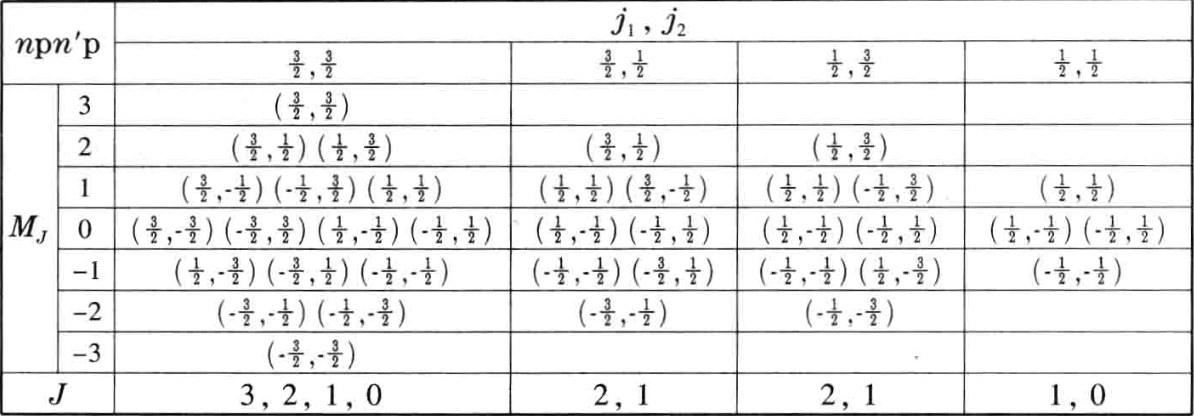
\includegraphics[scale=0.35]{fig/fig 5.8.png}
    \end{block}}
\uncover<2->{
    \begin{block}{$(n\mathrm{p})^2$}
        For equivalent electrons the Pauli exclusion principle restricts the states.
        \begin{center}
            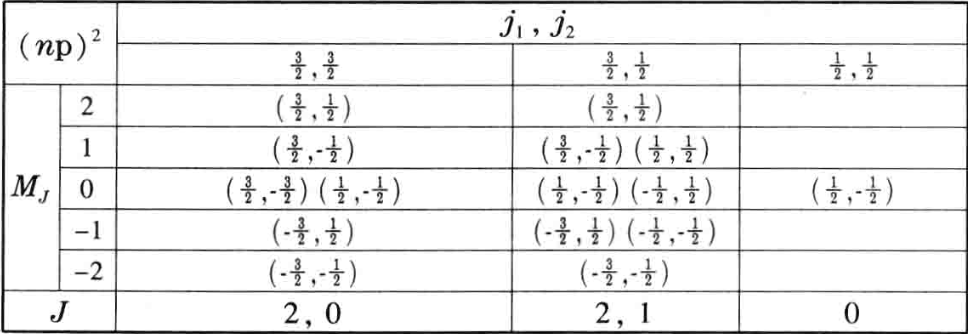
\includegraphics[scale=0.35]{fig/fig 5.9.png}
        \end{center}
    \end{block}}
\end{frame}